\section{编译器特性笔记}
\subsection{关于versioncheck原理优化代码原理}
Q:编译器代码优化是按照c文件为单位还是以函数为单位,如果以函数为单位,为什么类似于文件系统这些是以version\_check函数调用时,整个c文件的函数都会被调用进来?
\begin{itemize}
\item 函数链接是以\_entry标号作为入口,如果一个函数被显示调用,会把这个函数标号加进来链接,链接是以.o为单位,如果一个函数被显示调用,会把该函数的全部标号拉进来链接(包括结构体),如果一个结构体定义了\emphasizebox{used}属性,该标号会被最终链接进来,导致结构体里的函数指针也会被链接进来,这是使用version\_check选择性链接的原理。

\item libc.a这个库比较特殊,一个函数就是一个.o文件。


\end{itemize}

\subsection{C内联汇编}
参考: \myurlfootnote{https://www.ibiblio.org/gferg/ldp/GCC-Inline-Assembly-HOWTO.html}{GCC-Inline-Assembly-HOWTO}

一般为而言,通过 asm(...) 、 \_\_asm\_\_(...) 、 asm volatile(...) 和 \_\_asm\_\_ volatile(...) 来包含汇编指令模板的字符串形式,如果有额外的约束,通过 : 来分割并指定。
\subsubsection{内联汇编模板}
\begin{myccode}
asm ("汇编模板"
 : /* 输出操作数列表, 可空 */
 : /* 输入操作数列表, 可空 */
 : /* 修改了的寄存器列表, 可空 */
 );

asm ("nop"); // 一条 nop 指令, 没有额外的约束
__asm__ ("nop"); // 同上
 asm volatile ("nop"); // 表示不要随便移动(调度) 这条指令的位置
__asm__ volatile ("nop"); // 同上
\end{myccode}

在一些情况下,在内联汇编中使用了一些指令,这些指令会修改特定的寄存器,这个时候就需要在修改了的寄存器列表里面指明。这是因为内联汇编本身是字符串,并不会被解析,所以编译器内部并不能知道内联汇编的语义(即修改了哪些寄存器、有什么输入输出、做了什么事情以及是否能够被任意移动位置)。所以、我们总是需要通过输出,输入还有修改列表来指定。值得注意的是,为了实现 C 语言的调用协议,一些寄存器被用作了特殊的用途,如使用的栈指针寄存器。

\begin{myccode}
// 下面的做法也是危险的, 因为 r0 被修改了, 但是没有指明
__asm__ volatile ("r0 = 0");
__asm__ volatile ("r0 = 0" : : : "r0"); // ok

//另外一些情况下, 我们可能不希望自己分配寄存器的使用, 可以让编译器分配, 这个是还有需要通过%来指明
u32 reg;
__asm__ volatile ("%0 = rets" : "=r"(reg));
printf("rets的值是 %x", reg);
 // 这个时候表示第0个操作数作为输出, 最终编译器会给%0分配一个寄存器,并替换%0。
\end{myccode}

上述例子中的 "=r"(reg) 表示,对应的内联汇编本体会输出一个结果,并且这个结果应该放置到一个寄存器中,即 "=r" 。而 (reg) 则表示,希望编译器绑定 reg 变量和保存结果的寄存器。这样我们可以而通过访问 reg 获取对应的值。

\subsubsection{多条内联汇编}
一些情况下,会需要写多条连续的内联汇编。这个时候正确的做法是,把这些内联汇编语句用一个 \_\_asm\_\_ 块来表示,而不是分开多个 \_\_asm\_\_ 。例如:
\begin{myccode}
// 定义一个宏, 希望能够清空r1, r0寄存器
// 一个错误的做法:
// 下面的做法有多种错误
// 1. 应该使用一个__asm__块来, 而不是分开多个。 否则它们之间可能会插入其它的指令。
// 2. 内联汇编本体中修改了r1, r0寄存器, 但是没有通过修改列表来说明。
#define MACCLR() __asm__ volatile ("r1 = 0"); __asm__ volatile ("r0 = 0")

// 正确一点的做法:
#define MACCLR() __asm__ volatile( \
"r1 = 0 \n\t" \
"r0 = 0 \n\t" \
: \ // 没有输出
: \ //没有输入
: "r1", "r0" \ // 修改了 r1, r0
);

// 更好一些的做法:
// pi32v2中有一条指令
#define MACCLR() __asm__ volatile ("r1_r0 = 0" : : : "r1", "r0");
\end{myccode}

\subsubsection{寄存器约束}
编译器来分配寄存器的时候,需要指定需要分配的寄存器类型,总结如下:
\begin{figure}[H]
\centering
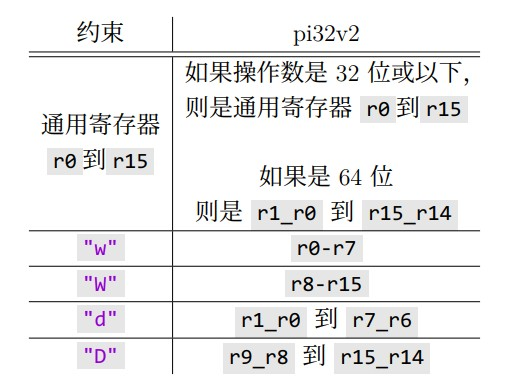
\includegraphics[scale=0.7]{asm_reg.jpg}
\caption{指定分配寄存器}
\label{fig:asm_reg}
\end{figure}
为了方便起见,对于一个 64 位寄存器 DR ,可以用 DR.l 来表示 DR 的低 32 位所在的寄存器, DR.h 用来表示 DR 的高 32 位所在的寄存器。例如r1\_r0.l表示r0,r1\_r0.h表示r1。

\subsubsection{输出约束}
有些时候,我们需要利用内联汇编来获取一些值,这些值需要输出到一些地方,我们通常需要一条输出约束。
\begin{myccode}
unsigned reg;
__asm__ volatile ("%0 = rets" : "=r"(reg));
printf("rets寄存器的值是: %x\n", reg);
// 由上面的汇编说明可以看到, 这个是 pi32v2 的汇编语法
// 表示 %0 表示第一个操作数, 这个是 : 后面开始算起的,
// "=r" 表示这个操作数需要写入到一个寄存器中,
// "=r"(reg) 表示, 输入的寄存器需要和 reg 分配到同一个
// 寄存器, 也就是可以认为把这个结果放入 reg
// 这个指令可以获取当前 rets 的值, 并放入 reg 变量中

__asm__ volatile ("%0 = sp\n" : "=r"(reg));
printf("sp寄存器的值是: %x\n", reg);
// 把 sp 的值存放在 reg 中
__asm__ volatile ("%0 = r4" : "=r"(reg));
printf("r4寄存器的值是 %x\n", reg);
// 获取 r4 的值到 reg 中

__asm__ volatile ("%0 = rets\n" : "=r"(reg));
printf("rets寄存器的值是 %x", reg);
\end{myccode}

\subsubsection{输入约束}
有些时候,我们需要指定一些输入到内联汇编中,这个时候,会需要一条输入约束。
\begin{myccode}
unsigned retaddr = get_retaddr();
__asm__ volatile ("reti = %0\n\t"
"rti \n\t" : : "r"(retaddr));
// "r" 表示这个操作数是被读的, 表示把 retaddr 的值赋值给
// reti, 然后执行 rti 指令, 实现了跳转
\end{myccode}

%值得注意的是,当有多于一条汇编指令需要内联的时候,通常我们写成上述形式,即每行一个汇编指令,并在末尾加上\textbackslash n \textbackslash t,由于内联汇编实际上以字符串形式存储,所以\textbackslash n \textbackslash t 表示换行并插入一个 tab 键。

\subsubsection{earlyclobber 操作数}
编译器在给内联汇编分配寄存器的时候,整块内联汇编被当做一条具有特定输入和输出的指令。并不会关心其内在的含义。例如:
\begin{myccode}
int a, b;
__asm__ volatile (
"%0 = ~ %1\n\t"
: "=r"(a)
: "r"(b));

 //在分配寄存器的过程中, 上面的内联汇编块被当做了
 // <INLINEASM> outs{%0}, ins{%1}
 // 特定于这个例子来说, 如果后续代码不在继续使用 b的值, 而只是使用了a的值
 // 那下面的一些寄存器分配都是合理的
 // 分配方式一:
 // r0 = ~ r0 ; 因为 b 后续不在被使用了, 所以其寄存器可以被a占用
 // 分配方式二:
 // r1 = ~ r0 ; 当然, 也有可能a分配了其它的寄存器
\end{myccode}

另外一些时候,我们的内联汇编块中不会只有一条指令,那么指令之间可能会有先后执行的顺序。这种把所有指令当做一个整体的处理方式,可能会导致问题,例如下面的例子:

\begin{myccode}
int a1, a2;
int b1, b2;
__asm__ volatile (
" %0 = ~ %2\n\t"
" %1 = ~ %3\n\t"
: "=r"(a1), "=r"(a2)
: "r"(b1), "r"(b2)
 );

 // 假设 b2, b1都不在这条指令之后被使用
 // 同样的, 这里在分配寄存器的时候, 还是会被当做下面的东⻄
 // <INLINEASM> outs{%0, %1}, ins{%2, %3}
 // 显然, 如果这个内联块能够作为一条指令整体执行完,
 // 那么下面的一些寄存器分配都是合理的
 // 分配方式一:
 // <INLINEASM> outs{r0, r1}, ins{r0, r1}
 // 即
 // r0 = ~ r0
 // r1 = ~ r1
 // 分配方式二:
 // <INLINEASM> outs{r1, r0}, ins{r0, r1}
 // 即
 // r1 = ~ r0
 // r0 = ~ r1
 // 但是这里, 第二种方式会导致错误的代码
\end{myccode}

上面的例子中,第二种分配方式,如果从一条指令的情况来看,是合理的。毕竟所有的输入一次性使用完毕,然后同时所有的输出被赋值完毕。但是问题在于,输入并不是一次性使用完毕,输出也不是一次性赋值完毕。而是使用一些输入(这里来说,就是第一条 not 指令),然后定义了一些输出,然后又使用了一些输入(这里来说,就是第二条 not 指令),再定义了一些输出。所以,我们需要一个方式标记一些输出,告知编译器这些输出被赋值的时候,还有一些输入没有被使用完,所以,不要让这些输出所使用的寄存器占用输入所使用的寄存器。这种标记方式就是\& 。上面的例子需要修正为

\begin{myccode}
int a1, a2;
int b1, b2;
__asm__ volatile (
" %0 = ~ %2\n\t"
" %1 = ~ %3\n\t"
: "=&r"(a1), "=r"(a2)
: "r"(b1), "r"(b2)
);
// 假设 b2, b1都不再这条指令之后被使用
// & 表示 a1 定义的时候, 输入还没有使用完毕, 也就是说
// 不应该把 a1 定义到 b2, b1 占用的寄存器上
// 对于 a2, 因为 a2 已经是最后一个定义的寄存器, 可以不用加上&
// 因为定义a2的时候, 所有的输入已经使用完毕了
// 当然, 加上也是可以的
\end{myccode}

\subsubsection{输入的同时是输出}
有些操作数是既有读属性,又有写属性的:比如一个后加指令的基地址寄存器,在访问内存后,基地址寄存器的值会被更新,对于这些指令,我们需要两条约束来指定。
\begin{myccode}
void t2sos16(short *in, short *out, int *coeff, int *mem, int npoint, intdstep) 
{
    const int coeffQ = 20;
    const int LeftBit = 8;
    int tmp32_1, tmp32_2, tmp32_3;
    long long tmp64_1;
    asm volatile (
    " %0 += 2<<2 \n\t"
    " %7 = %7 << 1 \n\t"
    "1: \n\t"
    " \n\t"
    " %1 = h[%8++=0] * [%0++=1<<2] (s) \n\t"
    " %4 = %1 >> (%20-%21) (s) # %5 = [%3+0] \n\t"
    " %5 += %4 \n\t"
    " %1 = [%0++=-3<<2] * %4 (s) \n\t"
    " %1 += [%0++=4<<2] * %5 (s) \n\t"
    " %1.l = %1 >>> %20 (up) # %6 = [%3+1<<2] \n\t"
    " %6 += %1.l \n\t"
    " %1 = [%0++=-3<<2] * %4 (s) \n\t"
    " %1 += [%0++=1<<2] * %5 (s) \n\t"
    " %1.l = %1 >>> %20 (up) # [%3+0] = %6 \n\t"
    " %8 += %7 # [%3+1<<2] = %1.l \n\t"
    " %5 >>>= %21 \n\t"
    " %5 = sat16(%5) (s) \n\t"
    " h[%9++=%7] = %5 \n\t"
    " \n\t"
    "if (--%2!=0) goto 1b \n\t"
     : "=&r"(coeff), // 第 0 个操作数, 对应于模板中的 %0
    "=&d"(tmp64_1), // 第 1 个操作数, 对应于模板中的 %1
    "=&w"(npoint), // 第 2 个操作数, 对应于模板中的 %2
    // w 约束了寄存器分配范围, 这是指令要求
    "=&w"(mem), // 第 3 个操作数, 对应于模板中的 %3
    "=&w"(tmp32_1), // 第 4 个操作数, 对应于模板中的 %4
    "=&w"(tmp32_2), // 第 5 个操作数, 对应于模板中的 %5
    "=&w"(tmp32_3), // 第 6 个操作数, 对应于模板中的 %6
    "=&r"(dstep), // 第 7 个操作数, 对应于模板中的 %7
    "=&r"(in), // 第 8 个操作数, 对应于模板中的 %8
    "=&r"(out) // 第 9 个操作数, 对应于模板中的 %9
    : "0"(coeff), // 表示这个操作数需要和 %0 操作数分配到同一个寄存器
    // 这是因为 %0 用作了后加访存指令的基地址操作数, 所以
    // %0 既是一个输入, 也是一个输出
    // "=r"(coeff) 说明了输出, "0"(coeff) 说明同时也是一个输入
    "1"(tmp64_1),
    "2"(npoint),
    "3"(mem),
    "4"(tmp32_1),
    "5"(tmp32_2),
    "6"(tmp32_3),
    "7"(dstep),
    "8"(in),
    "9"(out),
    "i"(coeffQ), // i 表示一个立即数
    "i"(LeftBit)
    :);
}
\end{myccode}

这个例子里面的 coeff 、 tmp64\_1 等,都是既需要读也许要写的操作数。 "=\&r" 表示对应的操作数在指令的输入寄存器使用完成之前就被修改了,这样编译器就不会把输入列表用到的寄存器分配给这些寄存器,这样标记不会导致一些寄存器分配的问题。值得注意的是, "0"(coeff) 之类的约束应该要放置到后面,以防影响操作数顺序。如下面的例子:
\begin{myccode}
int insert(int val_dst, int val_src, int pos, int len)
{
    int pat = (pos << 5) | len;
    __asm__ volatile (
    "%0 <= insert(%1, %2[12:8], %2[4:0])"
    : "=&r"(val_dst),
    : "r"(val_src),
    "r"(pat),
    "0"(val_dst) // 写在最后, 以防影响 %0, %1, %2 顺序
    );

    return val_dst;
}
\end{myccode}

\subsubsection{访问内存}
有时候,我们在内联汇编里面修改了内存,但是由于编译器不知道这个事实,将会导致一些问题。为了解决这个问题,我们需要 "memory" 约束。
\begin{myccode}
// "memory"
int *p = get_ptr();
put_u32hex(*p);
int np = *p + 1;
__asm__ volatile ("[%1] = %0"
: // 没有输出列表
: "r"(np), // 第零个操作数, 对应 %0
// 把 np 的值写入到 *p 的位置
"r"(p) // 第一个操作数, 对应 %1
 : "memory" // 表示内存被修改了
 );
 put_u32hex(*p); // 如果没有上面的 "memory" 可能这个的输出和上一个一样
\end{myccode}

当内联汇编修改了内存的时候,最好加上 "memory" ,这样编译器会失效掉一些缓存了的内存的值。例如上面的 *p ,不过不指定 "memory" 则编译器可能会缓存这个值(为了减少内存访问操作)。

一些例子:
\begin{myccode}
int add(int a, int b)
{
    int c;
    __asm__ volatile (
    "%0 = %1 + %2"
    : "=r"(c) // %0
    : "r"(a), // %1
    "r"(b)); // %2

     // 即 c = a + b
     return c;
}

int add_mem(int *pa, int *pb)
{
    int a, b;
    __asm__ volatile (
    "%0 = [%2] \n\t"
    "%1 = [%3] \n\t"
    "%0 = %0 + %1 \n\t"

    :
    "=&"(a), // %0 输出, 且不能和输入同一个寄存器(⻅earlyclobber操作数)
    "=r"(b) // %1 输出, 可以和输入同一个寄存器
    // (因为定义 %1 的时候, 所有输入都已经使用完毕)
    : "r"(pa), // %2 只是输入
    "r"(pb) // %3 只是输入
);

// 实现了 return *pa + *pb;
return a;
}
\end{myccode}

\subsection{CLZ指令}
\begin{myccode}
    Rd = clz(Rm)
\end{myccode}
计算前导零的个数,即从最高位开始,连续出现的 0 的个数。如0xFFF,FFFF,执行该指令后Rd结果为4。

\subsection{常用汇编语句}
\subsubsection{读写csfr}
\begin{myccode}
 //打印调用函数入口
 void log_rets_value()
{
    int tmp;
    __asm__ volatile("%0 = rets" : "=r"(tmp));
    printf("rets = 0x%x", tmp);
}

static void enable_int(void)
{
    int tmp;
    __asm__ volatile("%0 = icfg" : "=r"(tmp));
    tmp |= 1 << 8;
    __asm__ volatile("icfg = %0" :: "=r"(tmp));
}

static void disable_int(void)
{
    int tmp;
    __asm__ volatile("%0 = icfg" : "=r"(tmp));
    tmp &= ~(1 << 8);
    __asm__ volatile("icfg = %0" :: "=r"(tmp));
}
\end{myccode}
